\begin{frame}{Fact 1: there is substantial variation in the gender gap across CZ} 
\begin{figure}[!h]
\centering
\caption{The gender gap in the US in 2020}
\label{fig:gap_map2020}
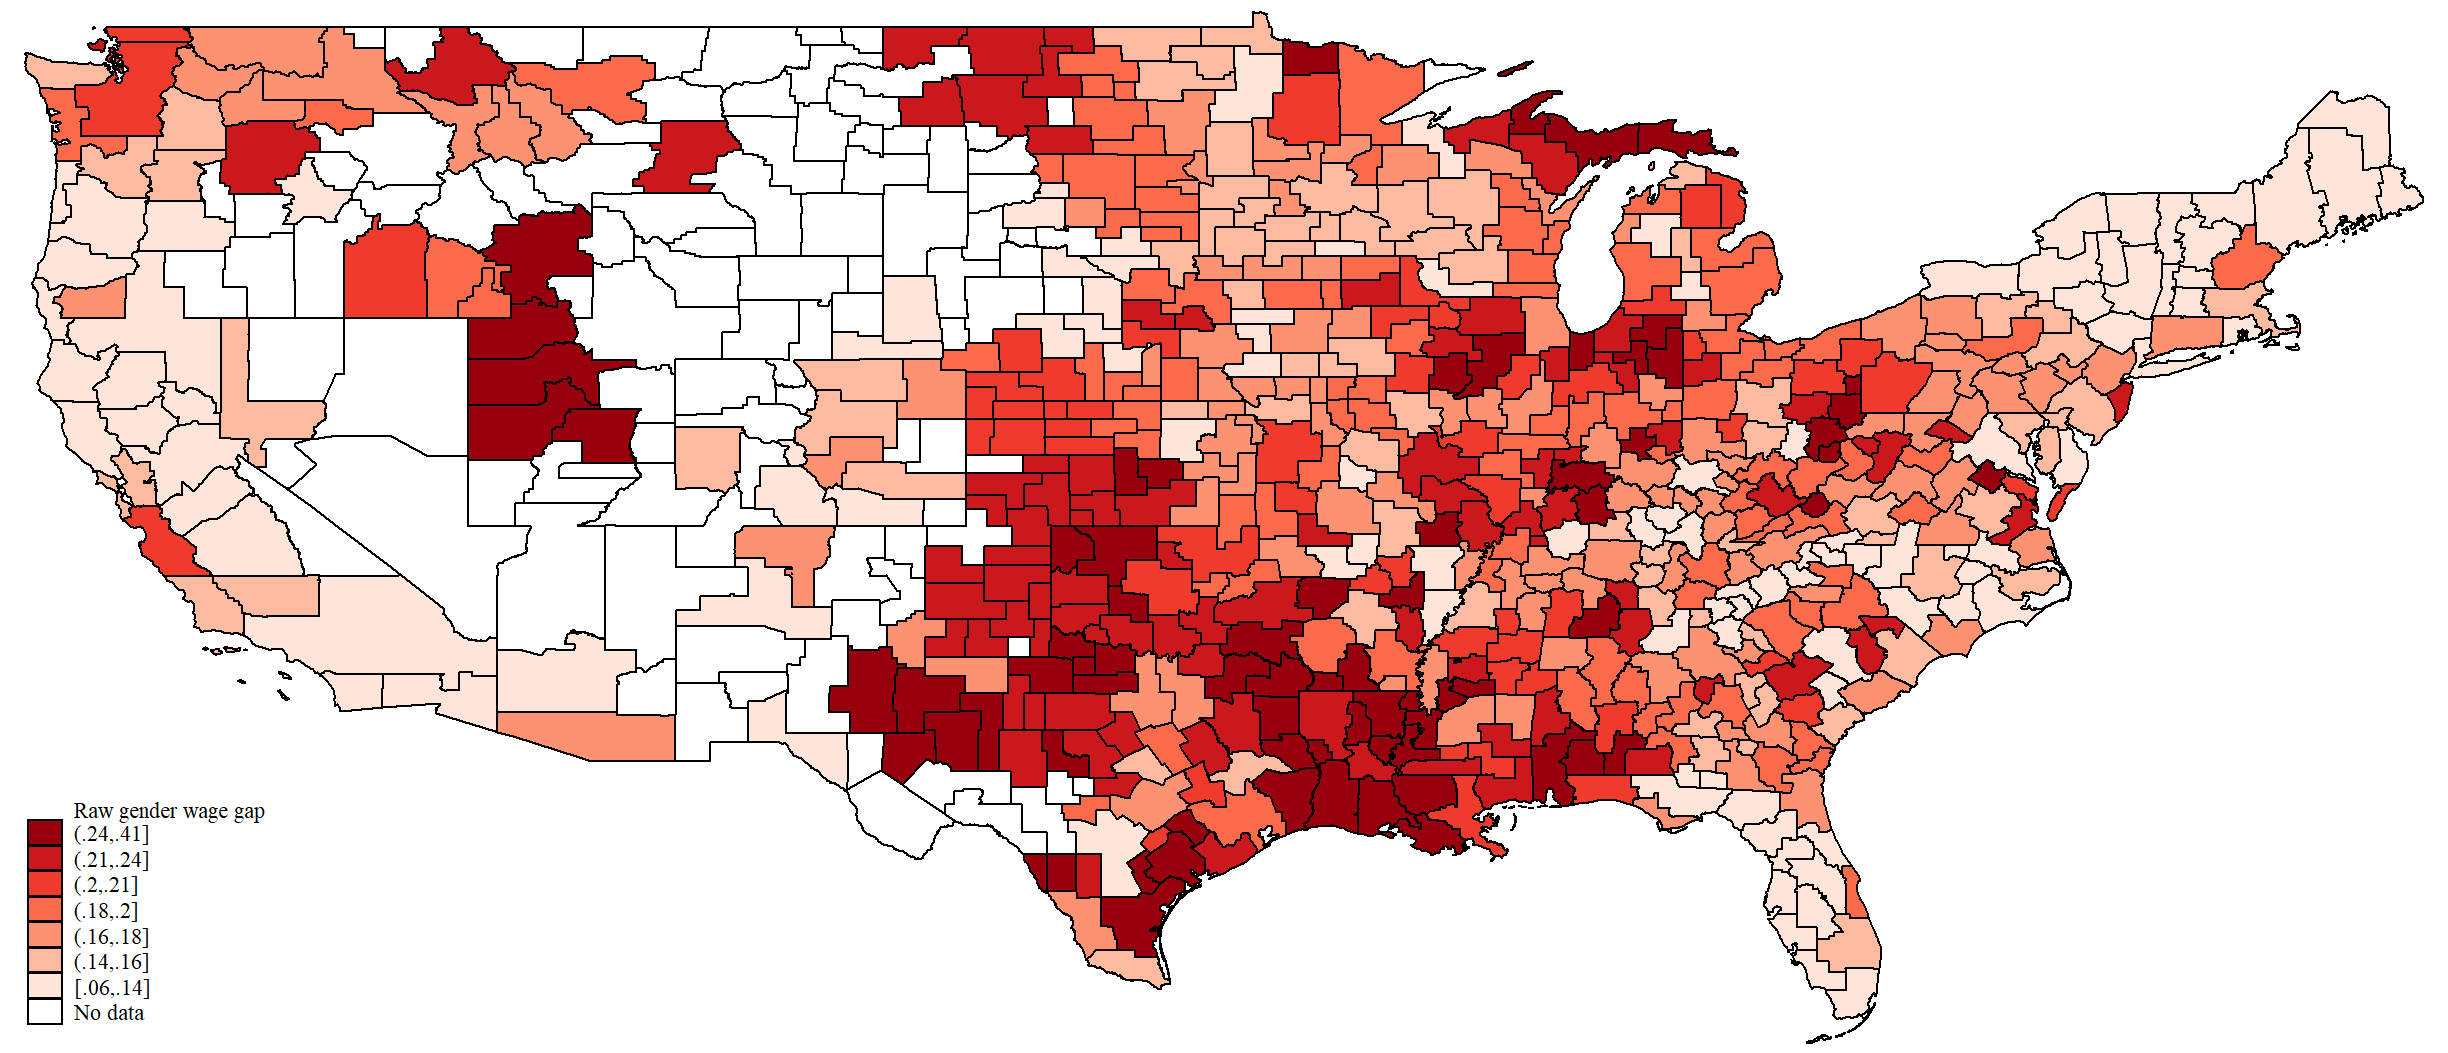
\includegraphics[width=1\textwidth]{../2_analysis/output/figures/raw_wage_map2020_full_time}
\par \begin{minipage}[h]{\textwidth}{\tiny\textbf{Note:} darker colors denote higher relative wages for men. Figure restricts to czones with population densities above 1 person per km$^2$ and full-time year-round workers.}\end{minipage}
\end{figure}

\end{frame}
\begin{frame}{Fact 1: Cross-CZ variation persists despite general decline at the national level}
	\begin{figure}[!h]
\centering
\caption{Evolution of raw gender gap across CZ}
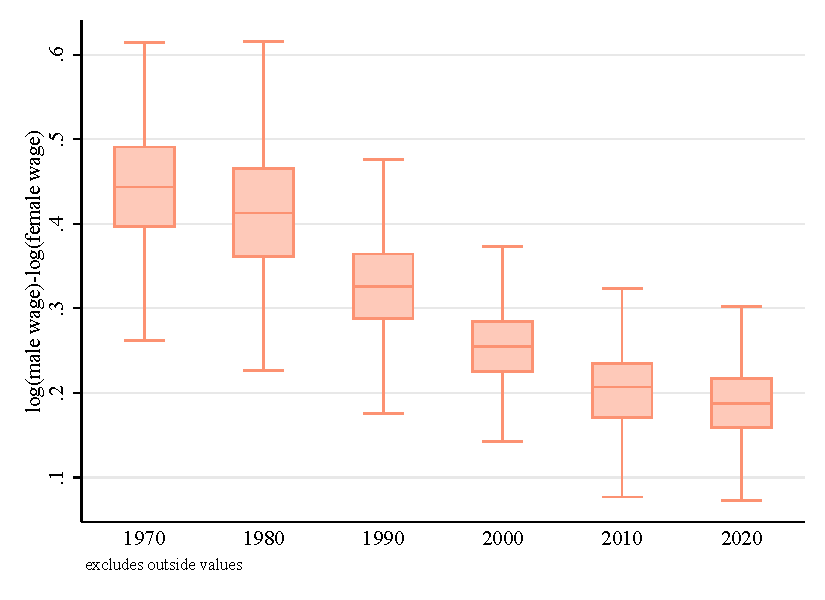
\includegraphics[width=.6\textwidth]{../2_analysis/output/figures/cz_gap_dispersion_full_time}
\par \begin{minipage}[h]{\textwidth}{\scriptsize\textbf{Note:} figure restricts to CZ with more than people per km$^2$ and full-time year-round workers..}\end{minipage}
\end{figure}

\end{frame}
\begin{frame}{Cross-CZ gender gap differences are persistent}
	\textbf{\alert{Regression specification:}} $w^{men}_{rt}-w^{women}_{rt}=\alpha_{rt}+\beta_{t}(w^{men}_{rt-j}-w^{women}_{rt-j})$
	\begin{figure}[!h]
\centering
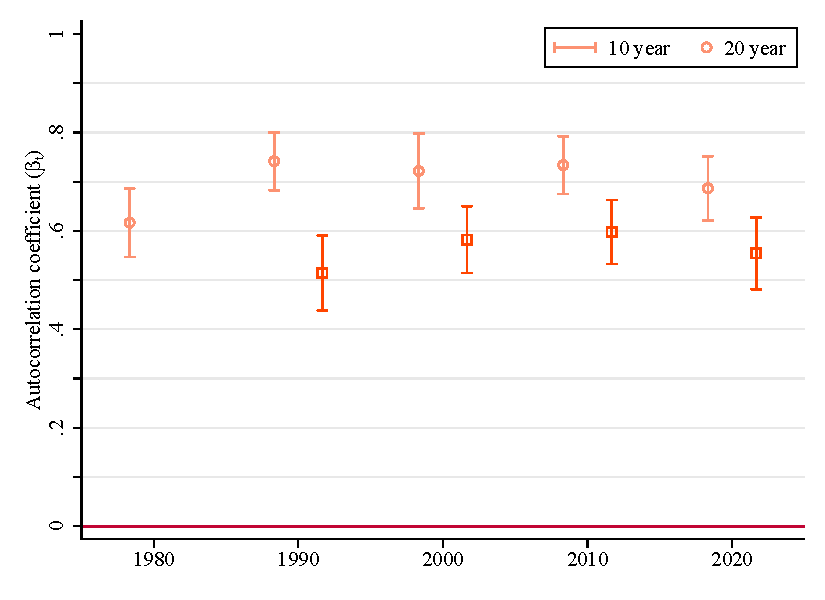
\includegraphics[width=.6\textwidth]{../2_analysis/output/figures/cz_gender_gap_persistence_full_time}
\par \begin{minipage}[h]{\textwidth}{\scriptsize\textbf{Note:} figure restricts to CZ with more than people per km$^2$ and full-time year-round workers.. Bars show 95\% robust confidence intervals. Standard errors are clustered at the CZ level. Dependent and independent variables are standardized}\end{minipage}
\end{figure}

\end{frame}
\begin{frame}{Fact 2: Denser CZ have faster declines in the gender wage gap}
	\begin{figure}[!h]
\centering
\caption{Change in male wage advantage in US CZ}
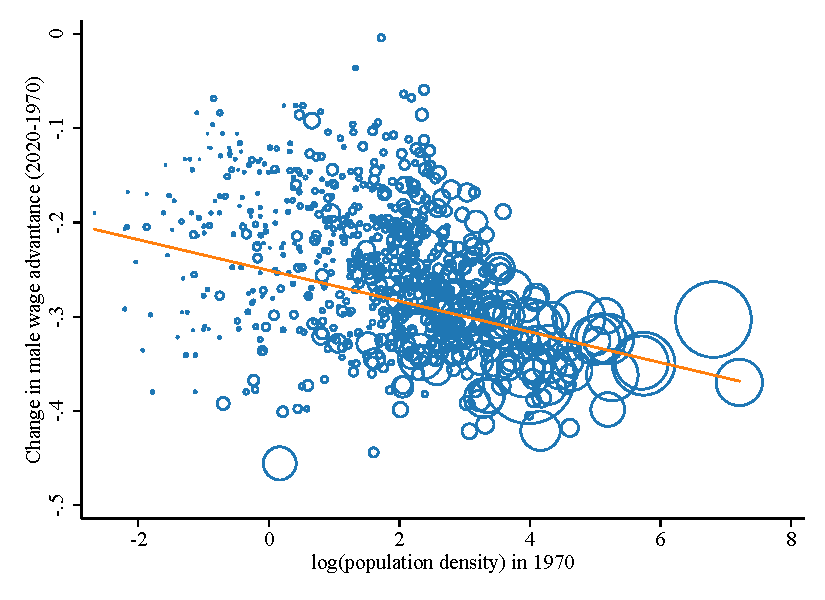
\includegraphics[width=.75\textwidth]{../2_analysis/output/figures/change_in_gap}
\end{figure}

\end{frame}
\begin{frame}{Fact 3: The gender gap - density relation has inverted}  
	\label{slide:baseline}
	\textbf{\alert{Regression specification:}}	$w^{men}_{rt}-w^{women}_{rt}=\alpha_{rt}+\beta_{t}\ln(density)_{rt}$
	\begin{figure}[!h]
\centering
\caption{Coefficient on population density $ \beta_t $}
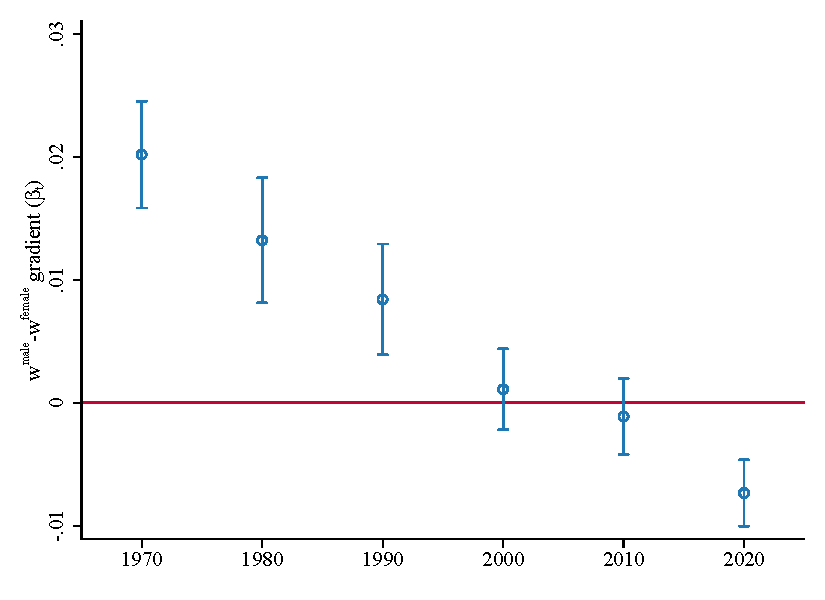
\includegraphics[width=.6\textwidth]{../2_analysis/output/figures/baseline_gradients_l_czone_density_full_time}
\par \begin{minipage}[h]{\textwidth}{\scriptsize\textbf{Note:} figure restricts to CZ with more than 1 people per km$^2$. Bars show 95\% robust confidence intervals.}\end{minipage}
\end{figure}

	\beamerbutton{\hyperlink{slide:distribution}{Distribution illustration}}
\end{frame}
\begin{frame}{How big are these coefficients?}  
		\begin{center}
\begin{threeparttable}[!h]
\caption{Male advantange changes implied by estimated elasticities}
\label{tab:IC}
\begin{tabular}{lcccccc}
\toprule
\toprule
\textbf{}&\multicolumn{1}{c}{\textbf{1970}}&\multicolumn{1}{c}{\textbf{1980}}&\multicolumn{1}{c}{\textbf{1990}}&\multicolumn{1}{c}{\textbf{2000}}&\multicolumn{1}{c}{\textbf{2010}}&\multicolumn{1}{c}{\textbf{2020}} \\
\midrule
Density elasticity $ (\beta ) $&       0.020         &       0.013         &       0.008         &       0.001         &      -0.001         &      -0.007         \\
 \hspace{3mm} s.d. wage gap &       0.073         &       0.077         &       0.060         &       0.049         &       0.049         &       0.050         \\
$ \hspace{3mm}\beta / sd $&       0.278         &       0.173         &       0.141         &       0.022         &      -0.023         &      -0.146         \\
\midrule IC range   &       0.029         &       0.019         &       0.013         &       0.002         &      -0.002         &      -0.012         \\
\hspace{3mm} (\% mean gap) &       0.065         &       0.047         &       0.040         &       0.007         &      -0.009         &      -0.064         \\
 \midrule 90 - 10 pctile range  &       0.061         &       0.040         &       0.027         &       0.004         &      -0.004         &      -0.025         \\
\hspace{3mm} (\% mean gap)&       0.137         &       0.097         &       0.082         &       0.014         &      -0.018         &      -0.133         \\
\bottomrule
\bottomrule
\end{tabular}
\begin{tablenotes}
\item \footnotesize \textit{Note:} changes based on unweighted estimated elasticities. Sample restricted to full-time year-round workers. Table generated on 28 Sep 2020 at 15:15:18.
\end{tablenotes}
\end{threeparttable}
\end{center}

\end{frame}
\begin{frame}{What can account for the change in the density-gradient?}
	\label{slide:controls}
	\textbf{\alert{Regression specification:}} $w^{men}_{rt}-w^{women}_{rt}=\alpha_{rt}+\beta_{t}\ln(density)_t$
	\begin{figure}[!h]
\centering
\caption{Coefficient on population density $ \beta_t $ controlling for worker characteristics}
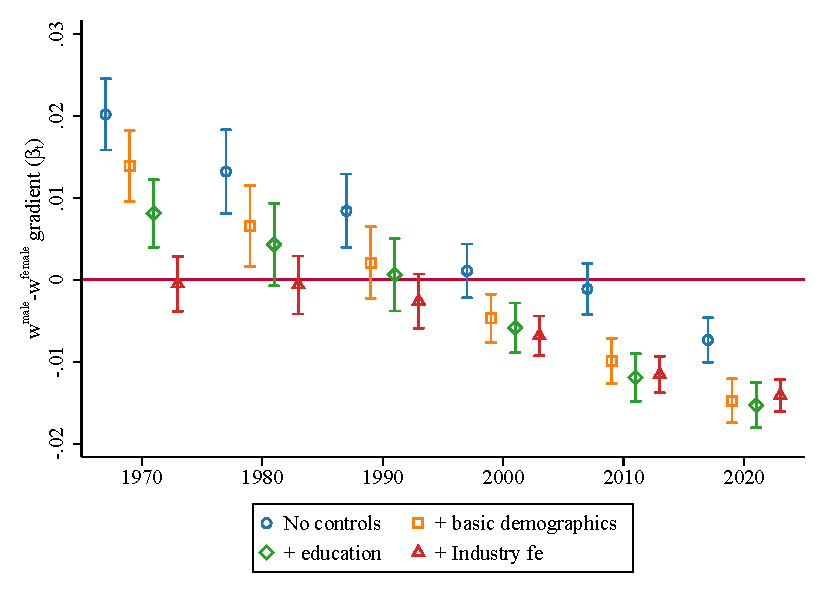
\includegraphics[width=.6\textwidth]{../2_analysis/output/figures/with_control_gradients_individual_l_czone_density_full_time}
\par \begin{minipage}[h]{\textwidth}{\tiny\textbf{Note:} figure restricts to CZ with more than 1 people per km$^2$. The regressions are done on data aggregated at the CZ level after residualizing individual-level characteristics. Bars show 95\% confidence intervals. Errors clustered at the CZ-level.}\end{minipage}
\end{figure}

	\beamerbutton{\hyperlink{slide:residual}{How do I control for individual characteristics?}}
\end{frame}